\documentclass[10pt]{article}
\usepackage[polish]{babel}
\usepackage[utf8]{inputenc}
\usepackage[T1]{fontenc}
\usepackage{amsmath}
\usepackage{amsfonts}
\usepackage{amssymb}
\usepackage[version=4]{mhchem}
\usepackage{stmaryrd}
\usepackage{graphicx}
\usepackage[export]{adjustbox}
\graphicspath{ {./images/} }

\title{OD SZKOLNIAKA DO ŻAKA }

\author{}
\date{}


\begin{document}
\maketitle
klasy 5 i 6 szkoły podstawowej\\
rok szkolny 2019/2020

\section*{Zadania - etap II}
Zadanie 1. Niech liczba a będzie rozwiązaniem równania:\\
(*) MCM - \(a=\mathrm{MCC}\),\\
zaś \(b\) niech będzie rozwiązaniem równania:\\
(**) MMCMIX + b = MMMCIX.\\
ile wynosi iloraz \(a: b\) ?

Zadanie 2. Basia w pewną sobotę spędziła przy komputerze 1,2 godziny, co stanowiło 0,125 dnia. Słońce tego dnia wzeszło o godzinie 7:03. O której godzinie był zachód słońca?

Zadanie 3. W puste kratki wstaw takie cyfry, aby liczba czterocyfrowa:

\[
a=\square 82 \square
\]

była podzielna przez 15.

Zadanie 4. Pewna liczba \(a\) przy dzieleniu przez 14 daje resztę 2. Inna liczba \(b\) przy dzieleniu przez 7 daje resztę 3. Jaką resztę przy dzieleniu przez 7 daje liczba \(3 a+5 b\) ?

Zadanie 5. Trójkąt ABC ma obwód 50 cm . Z wierzchołka C opuszczono na bok AB wysokość CD. Powstały dwa trójkąty: ADC i BDC o obwodach odpowiednio równych 30 cm i 36 cm . lle wynosi długość wysokości CD?\\
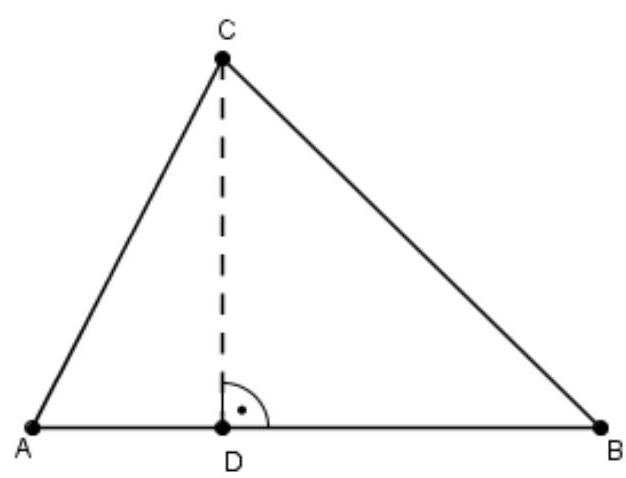
\includegraphics[max width=\textwidth, center]{2024_11_21_0dc2004b6b3d757b48b9g-1}


\end{document}